\chapter{Анализ данных о производительности сети}\label{ch:ch3}

\section{Сравнительный обзор и анализ платформ мониторинга и сбора показателей быстродействия интернет-сетей}\label{sec:ch3/sect1}

В настоящее время есть ряд систем, позволяющих собирать данные о работе мировой сети. Рассмотрим две наиболее известные и часто используемые в научных целях платформы - SamKnows и RIPE Atlas.

В начале рассмотрим платформу SamKnows. Она позволяет провайдерам, операторам связи и регуляторами проводить мониторинг производительности интернет сетей, в частности организация дает возможность измерять и анализировать качество соединения. Основанная в 2008 году, компания разработала уникальные решения для оценки производительности широкополосных сетей, используя как свое проприетарное специализированное оборудование - Whitebox (Рисунок \ref{whitebox}), так и программное обеспечение, позволяющее сделать измерительный зонд из маршрутизатора. 

Многие исследования подчеркивают точность проводимых измерений производительности в SamKnows \cite{Bagnulo2014Building}. Система использует методы, которые обеспечивают более точные и надежные данные о реальной производительности интернета. Это позволяет пользователям получать информацию о скорости загрузки, задержках и потере пакетов в реальных условиях \cite{Bajpai2015}, \cite{Sundaresan2012}.

Однако у платформы также есть и несколько проблем. Платформа носит коммерческий характер, поэтому некоторые функции платформы могут быть недоступны для обычных пользователей или требуют подписки на коммерческую версию, что ограничивает их использование в широких научных исследованиях или для анализа на уровне рядовых пользователей. Также присутствуют проблемы с конфиденциальностью данных, поскольку SamKnows собирает данные о сетевом трафике пользователей, существует риск утечек информации или нарушения конфиденциальности. Хотя платформа предпринимает шаги по обеспечению конфиденциальности, использование платформы может вызвать опасения у пользователей по поводу сбора личных данных.

\begin{comment}
	\begin{figure}[htbp]
		\centerfloat{
\includegraphics[scale=0.5]{whitebox}}
		\caption{Измерительное оборудование SamKnows - Whitebox \cite{samknows_web}}
		%https://samknows.one/hc/en-gb/articles/360000451757
		\label{whitebox}
	\end{figure}
\end{comment}

Еще одной из самых известных систем проведения измерений внутри сетевой инфраструктуры является платформа RIPE Atlas \cite{ripe}. На момент весны 2025  в системе зарегистрировано более чем 80 тысяч активных пользователей и подключено более 13 тысяч устройств в более чем 180 странах (карта покрытия отображена на Рисунке \ref{map}). Проект поддерживают и спонсируют крупные телекоммуникационные компании,  в частности ConsoleConnect, IPinfo,  COMCAST и La Poste. 

За более чем 13 лет существования были внедрены несколько аппаратных версии устройств, множество версий прошивок, а также появились программно-развертываемые зонды (программные или программно-аппаратные комплексы для проведения измерений). Система продолжает постоянно  модернизироваться и развиваться. Так, на текущий момент выпущена уже 5-я версия аппаратного зонда (Рисунок \ref{probev5}), который базируется на устройствах Turris Mox \cite{turris}.
Также регулярно выходят обновления и для программных зондов. 

\begin{comment}
	\begin{figure}[htbp]
		\centerfloat{
\includegraphics[scale=0.8]{probev5}}
		\caption{Пятая версия аппаратного зонда RIPE Atlas <<Probe V5>>}
		\label{probev5}
	\end{figure}
\end{comment}


\begin{figure}[htbp]
	\centering
	\begin{minipage}{0.49\textwidth}
		\centering
		
\includegraphics[width=\linewidth]{whitebox}
		\caption{Измерительное оборудование SamKnows - <<WhiteBox>>}
		\label{whitebox}
	\end{minipage}
	\hfill
	\begin{minipage}{0.49\textwidth}
		\centering
		
\includegraphics[width=0.77\linewidth]{probev5}
		\caption{Аппаратный зонд RIPE Atlas - Probe V5}
		\label{probev5}
	\end{minipage}
	
	
\end{figure}


Данная платформа была выбрана для применения в последующих исследованиях благодаря возможности регистрации каждого конкретного измерения и устройства, в отличие от системы мониторинга SamKnows, принадлежащей компании Cisco, которая предоставляет преимущественно агрегированные статистические данные (например, средние или медианные значения метрик) \cite{samknows}. Важно отметить, что платформа от компании Cisco характеризуется более строгим протоколом отбора участников и преимущественно коммерческой моделью взаимодействия.


В частности стоит отметить, что доступ к полноценной версии платформы SamKnows One возможен только по запросу через систему продаж или официального представителя компании. Этот аспект существенно снижает ее привлекательность по сравнению с платформой RIPE Atlas, которая является децентрализованной и более открытой.


Еще одним преимуществом работы с подобными системами является сбор данных из реальной сетевой инфраструктуры, а не смоделированного трафика или трафика, собранного с лабораторных стендов. Примером таковых являются наборы данных, предоставляемые Канадским институтом кибербезопасности (например набор данных CICDDoS2019 \cite{ddos}). 

Стоит подчеркнуть главное преимущество использования подобных систем - это сбор данных из реальной сетевой инфраструктуры, а не из смоделированного трафика или трафика, полученного с лабораторных стендов. Примерами таких наборов данных служат те, что предоставляются Канадским институтом кибербезопасности и были рассмотрены в главе \ref{ch:ch2}.

%Our research focuses on sample data collection, exploratory data analysis \cite{eda}, assessment of measurement bias, and clustering of collected data to reduce bias.


\begin{figure}[htbp]
	\centerfloat{
\includegraphics[width=1.0\linewidth]{map}}
	\caption{Карта покрытия измерительными зондами платформы RIPE Atlas}
	\label{map}
\end{figure}


\section{Особенности работы платформы RIPE Atlas }\label{sec:ch3/sect2}


В процессе работы с платформой RIPE Atlas было установлено, что одной из ключевых проблем, ограничивающих достоверность и воспроизводимость результатов сетевого анализа, являются систематические искажения, обусловленные неоднородностью аппаратно-программной инфраструктуры измерительных зондов \cite{ripe2}. В частности, значительные дополнительные задержки наблюдаются в устройствах первых двух версий, что свидетельствует о влиянии аппаратных характеристик на результаты измерений. Кроме того, различия в версиях прошивок могут приводить к непредсказуемым вариациям в измеряемых параметрах, внося дополнительный шум в данные. С точки зрения статистического анализа, распределение измеряемых сетевых признаков представляет собой смесь распределений, где результирующая плотность распределения формируется как взвешенная сумма плотностей, соответствующих различным типам и версиям зондов, каждый из которых характеризуется собственными параметрами распределения.

Другим значимым фактором, влияющим на точность измерений, является наличие перекрёстного трафика (или же кросс-трафика), искажающего оценки загрузки сетевых каналов. Поскольку платформа RIPE Atlas изначально ориентирована на мониторинг доступности сети, она не предусматривает предварительную оценку доступной пропускной способности перед проведением измерений. Тем не менее, косвенная оценка влияния перекрёстного трафика может быть осуществлена путём анализа временной динамики сетевых показателей. В частности, сопоставление данных, собранных в разные временные интервалы суток, позволяет выявлять корреляции с типичными пиковыми нагрузками, что даёт возможность формулировать гипотезы о характере и степени искажений, вносимых сторонним трафиком.

Дополнительным аспектом, требующим учёта при обработке и подготовке наборов данных, является циклическая активность отдельных зондов, обусловленная их эксплуатационными режимами. Наблюдения показывают, что некоторые устройства демонстрируют регулярные суточные паттерны включения и выключения (например, активируются в 10:00 и отключаются в 18:00). Такое поведение может приводить к систематическим пропускам данных и смещению выборки, что необходимо учитывать при построении моделей сетевой активности и интерпретации результатов анализа.

%%%%%%%%%%%%%%%%

Взаимодействие с рядовыми пользователями основано на использовании системы баллов. Внося вклад в систему путем установки/инициализации зондов, пользователи могут запросить выполнение собственных измерений с использованием накопленных со временем баллов.

Система RIPE Atlas позволяет проводить множество типов измерений. Например:
\begin{itemize}
	\item PING - время отклика конечного адреса назначения
	\item TRACEROUTE - путь и время соединения между промежуточными адресами между источником и  адресом назначения
	\item DNS - данные процесса получения IP-адресов от DNS-серверов
	\item TLS - данные работы сертификатов безопасности
	\item HTTP - данные обработки http-запросов
	\item NTP - данные об отслеживании процесса синхронизации часов в сети
\end{itemize}


Различные типы измерений требуют разного количества кредитов (таблица \ref{prices}), а стоимость также зависит от параметров (частота, длительность и т. д.). Результаты предоставляются в формате json через API платформы или веб-интерфейс.


\begin{table}[htbp]
	\caption{Стоимость в баллах различных измерений в расчете на один запрос к одному зонду}
	\begin{center}
		\begin{tabular}{|c|>{\centering\arraybackslash}p{7cm}|}
			\hline
			\textbf{Вид измерений} & \textbf{<<Цена>> в баллах в расчете на единичное измерение} \\
			\hline
			TRACEROUTE & 60 \\
			\hline
			DNS (UDP) & 20 \\
			\hline
			DNS (TCP) & 40 \\
			\hline
			TLS & 20 \\
			\hline
			PING (ipv4/ipv6) & 6 \\
			\hline
			NTP & 20 \\
			\hline
			HTTP & 20 \\
			\hline
		\end{tabular}
		\label{prices}
	\end{center}
\end{table}



В связи с наличием различных типов и версий устройств в данных может наблюдаться неоднородная картина распределений метрик. Пример таковых был обнаружен в ходе анализа данных измерения типа TRACEROUTE до сервера gov.ru. Измерение содержит 480 различных зондов с различными 8 версиями прошивок и 8 версиями программного обеспечения. Устройства разделяются на несколько классов: аппаратные зонды (которые разделяются на 5 разных версий устройств), устройства типа <<Якорь>> (Anchor) и  программные зонды (т.е. программные реализации зондов).

Аппаратные датчики V1 и V2 представляют собой специальное оборудование, созданное на основе модуля Lantronix XPort Pro, в то время как датчики v3 представляют собой стандартные беспроводные маршрутизаторы TP-Link, работающие под управлением прошивки OpenWrt5. 

Датчики версии V4 построены на базе одноплатного компьютера NanoPi NEO Plus2, оснащённого операционной системой Linux \cite{ripeweb}. С точки зрения аппаратных характеристик, датчики версии V3 обладают более высокой производительностью по сравнению как с устаревшими моделями V1 и V2, так и с V4. Кроме того, измерения могут выполняться не только на стандартных датчиках, но и на так называемых «Якорях» — выделенных серверах с повышенными вычислительными возможностями и стабильным сетевым подключением. Это существенно расширяет гетерогенность используемого оборудования и, как следствие, увеличивает вариативность измеряемых параметров.

На рисунке \ref{probe_offset} представлена картина распределений времени отклика первого узла маршрутизации (то есть домашнего шлюза) в течение двух суток для всех доступных аппаратных версий датчиков. Теоретически, задержка на первом сетевом переходе в локальной сети не должна превышать 1 мс при нормальных условиях функционирования. Полученные данные демонстрируют значительное влияние аппаратной версии датчика на результаты измерений: большинство датчиков V3, V4, а также якорей и программных зондов показывают задержку ниже порога в 1 мс. В то же время, датчики V1 и V2 систематически демонстрируют повышенные значения задержки на первом переходе, превышающие 1 мс, при средней разнице порядка 1,5 мс и более. Это указывает на наличие систематического смещения, связанного с устаревшей или менее производительной аппаратурой.

В выборку также включены данные по датчикам версии V5. Однако, учитывая их недавнее внедрение (по состоянию на 2024 год), объём представленных измерений крайне ограничен — в ходе анализа был зафиксирован лишь один экземпляр устройства V5. В силу недостаточного объёма статистики, данные по V5 исключены из дальнейшего рассмотрения, поскольку их включение не позволит провести репрезентативный и достоверный анализ.

В ходе анализа распределения времени отклика для первого узла, был отмечен значимый сдвиг для V1, V2 и V4 относительно V3, программных зондов и зондов типа Anchor. И в то же время, хотя распределения для Anchor и V3 имеют статистически значимое различие (вероятность получить такие же или ещё большие отклонения при условии нулевой гипотезы (здесь и далее для краткости p-value) p-value $\ll$ 0,05 по тесту Манна–Уитни), их численное различие имеет незначительный характер с практической точки зрения - менее 0,01 мс, поэтому для них не видится необходимость в предобработке данных, однако стоит отметить, что это может потребоваться для измерения, содержащего большее количество устройств типа Anchor. Также стоит отметить, что тот же вывод можно сделать и для устройств с разными версиями прошивки.

Стоит подчеркнуть, что в последних измерениях на платформе наблюдается незначительная доля старых версий прошивок (менее 5 \%) и  основная масса устройств одной аппаратной версии имеют одну прошивку, поэтому исследование было сосредоточено именно на влиянии различных аппаратных реализаций.


\begin{figure}
	\centering
	
\includegraphics[width=0.9\linewidth]{probe_offset.png}
	\caption{Распределение времени отклика до первого узла маршрута в зависимости от типа устройства}
	\label{probe_offset}
\end{figure}


\section{Калибровка получаемых значений времени отклика}\label{sec:ch3/sect3}


Для решения проблемы наличия искажений в получаемых показателях можно предложить несколько решений: 
\begin{itemize}
	\item Фильтрация зондов. То есть удаление старых версий устройств, которые добавляют дополнительную задержку
	\item Мультимодальный анализ. Использование разных методов обработки и анализа результатов с разных версий зондов.
	\item Калибровка. Устранение искажений в получаемых показателях.
\end{itemize} 
И для лучшего понимания картины работы сети и сохранения объема данных предпочтительно последнее. Простым вариантом может служить коррекция систематической погрешности на основе медианных оценок. Данный подход заключается в оценке смещения в распределениях RTT до первого узла для версий V1, V2 и V4, интерпретируемого как систематическая ошибка измерений. Полученное значение смещения, определяемое как медианное отклонение от эталонного распределения, последовательно вычитается из исходных данных с целью центрирования распределений:

% пример формулы
\begin{equation}
	latency^{*} = latency + systematic\_error
	\label{error}
\end{equation}

\begin{figure}
	\centering
	
\includegraphics[width=0.9\linewidth]{simple_calib.png}
	\caption{Результат калибровки RTT до первого узла маршрута}
	\label{rtt_after}
\end{figure}

Итак, влияние оборудования можно исправить таким образом, но стоит отметить, что в выборке присутствуют также есть программные зонды. Также стоит отметить, что и устройства типа Anchor обладают отличной от остальных зондов формой распределения. К сожалению, программные устройства трудно калибровать из-за большого разнообразия устройств, на которые пользователи могут установить программное обеспечение RIPE. Этот аспект требует дальнейшего исследования, которое будет проведено в последующих разделах данной работы.


Как можно отметить из Таблицы \ref{calib1} - результаты статистических тестов не изменились до пороговых уровней (p-value не перешло за порог 0,01). Однако визуально и в значениях статистик наблюдается положительная динамика. Можно сделать вывод о необходимости использования более детального метода калибровки. В частности на это подталкивают значимые различия в дисперсии наблюдаемых картин.


\begin{table*}[!ht]крово
	\centering
	\caption{Результаты калибровки, выраженные в показаниях статистических тестов Манна–Уитни (U-test) и Колмогорова–Смирнова (KS-test). U/D - значение статистики в тестах}
	\begin{tabular}{|c|c|c|c|c|c|c|c|}
		\hline
		Стат. & \multirow{3}{*}{Этап} & \multicolumn{6}{c|}{Тип калибруемого устройства} \\ \cline{3-8}
		Тест & & \multicolumn{2}{c|}{System V1}
		& \multicolumn{2}{c|}{System V2} 
		& \multicolumn{2}{c|}{System V4} \\ \cline{3-8}
		& & U/D & p-value
		& U/D & p-value
		& U/D  & p-value \\ \hline
		KS-test & До     & 1,0        & 0,0        & 1,0         & 0,0                  & 0,89    & 0,0        \\ \hline
		KS-test & \textbf{После}  & 0,249      & 2,6e-42    & 0,23        & 5,7e-124    & 0,058   & 4,5e-19    \\ \hline
		U-test  & До     & 13e6       & 0,0        & 53e6        & 0,0                  & 168e6   & 0,0        \\ \hline
		U-test  & \textbf{После}  & 6e6        & 0,0003     & 24e6        & 1,8e-14     & 85e6    & 0,0008     \\ \hline
	\end{tabular}
	\label{calib1}
\end{table*}




Исходя из статистических тестов и визуального отображения получаемой картины распределений собираемых показателей с различных версий устройств можно заключить что распределения с устройств Software и Anchor значимо отличают от других не только по дисперсии, но и по форме функций плотности распределения. Поэтому был сделан вывод о необходимости разработки методов преобразования распределений (Distribution Transforming).
 

\section{Преобразование распределений (Distribution transforming)}\label{subsec:ch3/sect4}

Как было упомянуто в предыдущем разделе для полноценной калибровки возникает необходимость в применении методов преобразования распределений. Одним из подходов, который можно применить для данной задачи - перевод исследуемых выборок в одинаковое пространство распределений (Рисунок \ref{fig:calibration}). Например таковым может быть нормально или равномерное распределения. Однако стоит подчеркнуть, что в наших данных присутствуют выбросы, а так же они имеют скошенный характер и ограниченны слева (время отклика не может быть $<0$). Поэтому классический подход с использованием Z-нормализации не подойдет:

\begin{equation}
	z =  \frac{x - \mu}{\sigma} ,
	\label{z_tr}
\end{equation}
где $z$ – результат преобразования, $x$ – исходные данные, $\mu$ – оценка среднего значения, $\sigma$ – оценка стандартного отклонения.

\begin{figure}[ht]
	\centerfloat{
		
\includegraphics[scale=0.6]{time_series/calibration_ru}
	}
	\caption{Концептуальная схема разрабатываемого метода калибровки}\label{fig:calibration}
\end{figure}


Одним из подходящих методов для калибровки исследуемых данных является квантильтрансформер (QuantileTransformer). Это метод, доступный в библиотеке scikit-learn и используемый для преобразования числовых данных в соответствии с другим распределением, часто равномерным или нормальным (гауссовым). Это форма преобразования данных, которая может быть особенно эффективна при работе с ненормально распределенными данными или в тех случаях, когда для последующих моделей полезно использовать нормально распределенные признаки \cite{MingXuan_2023_01, Varoquaux_2015_06}. %Пример применение восстановления распределения после деформации изображен на Рисунке \ref{fig:qt1}.

\begin{comment}
	\begin{figure}[ht]
		\centerfloat{
			\hfill
			\subcaptionbox{Исходный вид выборки}{%
				
\includegraphics[width=0.33\linewidth]{qtransf/ref_sample}}
			\hfill
			\subcaptionbox{Выборка после линейной деформации}{%
				
\includegraphics[width=0.33\linewidth]{qtransf/deform_sampe}}
			\hfill
			\subcaptionbox{Калибровка квантильтрансформером}{%
				
\includegraphics[width=0.33\linewidth]{qtransf/Gamma-dist}}
			\hfill
		}
		\caption{Пример применения квантильтрансформера}\label{fig:qt1}
	\end{figure}
\end{comment}


Для исследования эффективности было проведено исследование на синтетических данных. Использовалось гамма-распределение (\ref{gamma}) и линейные деформации, близкие к наблюдаемым в полученных данных при сравнении разных типов устройств. Для определения оптимальных параметров проводилось исследование метрики MAPE для набора параметров моделей и разных генераций. В ходе чего были определены оптимальные значения количества квантилей для эталонной выборки и восстанавливаемой: 24 и 43 квантиля при объеме выборок 1000 и 500 соответственно. 

\begin{equation}
	f(x) =  x^{k-1} {{e^{-x/\theta}}\over{\theta^k \Gamma(k)}}
	\label{gamma}
\end{equation}

C такими параметрами калибровка была применена к реальным данным со схожими объемами выборок (отличие объемов <5\%). Как визуально так и по метриками выборок наблюдается сдвиг в сторону эталонного устройства (Рисунки \ref{fig:qt2} и \ref{fig:qt3}). Устройство версии V3 было выбрано как эталонно в силу его наибольшей аппаратной мощности и минимальным показателям среднего времени отклика.

\begin{figure}[ht]
	\centerfloat{
		\hfill
		\subcaptionbox{Исходный вид выборки эталонного и калибруемого устройства}{%
			
\includegraphics[width=0.49\linewidth]{qtransf/test_before}}
		\hfill
		\subcaptionbox{Выборка после калибровки с параметрами, подобранными на синтетических данных}{%
			
\includegraphics[width=0.49\linewidth]{qtransf/test}}
		\hfill
	}
	\caption{Пример применения квантильтрансформера на данных RIPE Atlas}\label{fig:qt2}
\end{figure}


\begin{figure}[ht]
	\centerfloat{
		\hfill
		\subcaptionbox{Исходный вид выборки эталонного и калибруемого устройства (лог. масштаб)}{%
			
\includegraphics[width=0.49\linewidth]{qtransf/test_before2}}
		\hfill
		\subcaptionbox{Выборка после калибровки с параметрами, подобранными на синтетических данных (лог. масштаб)}{%
			
\includegraphics[width=0.49\linewidth]{qtransf/test2}}
		\hfill
	}
	\caption{Пример применения квантильтрансформера на данных RIPE Atlas(логарифмический масштаб)}\label{fig:qt3}
\end{figure}


\begin{table}[!ht]
	\caption{Изменение статистик в ходе калибровки полученных данных}
	\centering
	\begin{tabular}{|c|c|c|c|}
		\hline
		Статистика & Данные V3 & Данные V4 & \makecell{Данные V4 \\ после калибровки} \\ \hline
		min & 0,308 & 0,677 & 0,308  \\ \hline
		median & 0,472 & 0,920 & 0,474  \\ \hline
		max & 2,760 & 2,777 & 2,760  \\ \hline
	\end{tabular}
\end{table}

Несмотря на в целом положительный результат метод явно требует доработки и обобщения на всю массу имеющихся данных. Также он является довольно трудоемким в виду необходимости в подборе оптимального количества квантилей для обоих выборок и с ростом разнообразия устройств в системе измерений этот аспект будет усложнять применимость метода. Поэтому в дальнейшей работе от этого подхода было решено отказаться.


\section{Преобразование распределений с использованием приближений параметрическими распределениями}\label{subsec:ch3/sect5}

В ходе более детального анализа полученных данных было отмечено, что хотя тип Anchor и system: V3 не имеют значимых различий согласно критерию Манна-Уитни, визуально можно отметить их отличие по форме распределений. Схожие методы можно сделать и для типа Software. Также стоит подчеркнуть, что устройства в выборке расположены в различных городах, в сетях разных провайдеров и в разных ASN (autonomous system number) можно сделать вывод о связи доп задержки в первую очередь с самими устройствами измерения, а не особенностями структуры сети.
	

Данный аспект подводит к необходимости более комплексного подхода к калибровке, нежели простой анализ средних или медианных показателей. В связи с этим был разработан и изучен подход с использование параметрических распределений. 


\subsection{Подбор параметрического распределения для оценки наблюдаемых данных}\label{subsec:ch3/sect5/sub1}

В ходе анализа полученных данных были проведены статистических тесты для определения характера генеральной совокупности для выборок времени отклика. Однако результаты тестов Шапиро-Уилка и $\chi^2$-тест, не позволяют принять гипотезу о принадлежности выборок к нормальной, логнормальной или гамма-распределенной генеральной совокупности. Поэтому было принято решение о необходимости проведения оценки картин распределения путем оценочных методов. 

Для выборки, полученной с каждого типа устройства были получены оценки функции плотности вероятности (далее pdf) с помощью метода ядерной оценки плотности распределения (KDE-kernel density estimation). Для получения данной оценки использовался пакет scipy и следующие параметры: типа ядра – Гауссово, метод оценки ширины полосы – правило Скотта. Метод был выбран на основе рекомендаций работ \cite{Holterbach2015, ripe_miss, ripe2}. Результаты оценки приведены на Рисунке \ref{fig:kde}.

\begin{figure}
	\centering
	
\includegraphics[width=0.75\linewidth]{calib/kde}
	\caption{KDE-оценка плотности вероятности времени отклика для различных типов устройств}
	\label{fig:kde}
\end{figure}

Далее были получены оценки параметров для ряда распространенных <<табличных>> распределений: 

\begin{itemize}
	\item нормальное (normal)
	\item логнормального (lognorm)
	\item «смещенное» нормальное (оно же - skew normal distribution, skewnorm)
	\item обобщённое нормальное (gennorm) 
	\item гамма (gamma)
\end{itemize}

%Пример одной из полученных оценок можно увидеть на Рисунке \ref{fig:examplekde} в Приложении \ref{app:1} на примере гамма-распределения.

\begin{comment}
	\begin{figure}
		\centering
		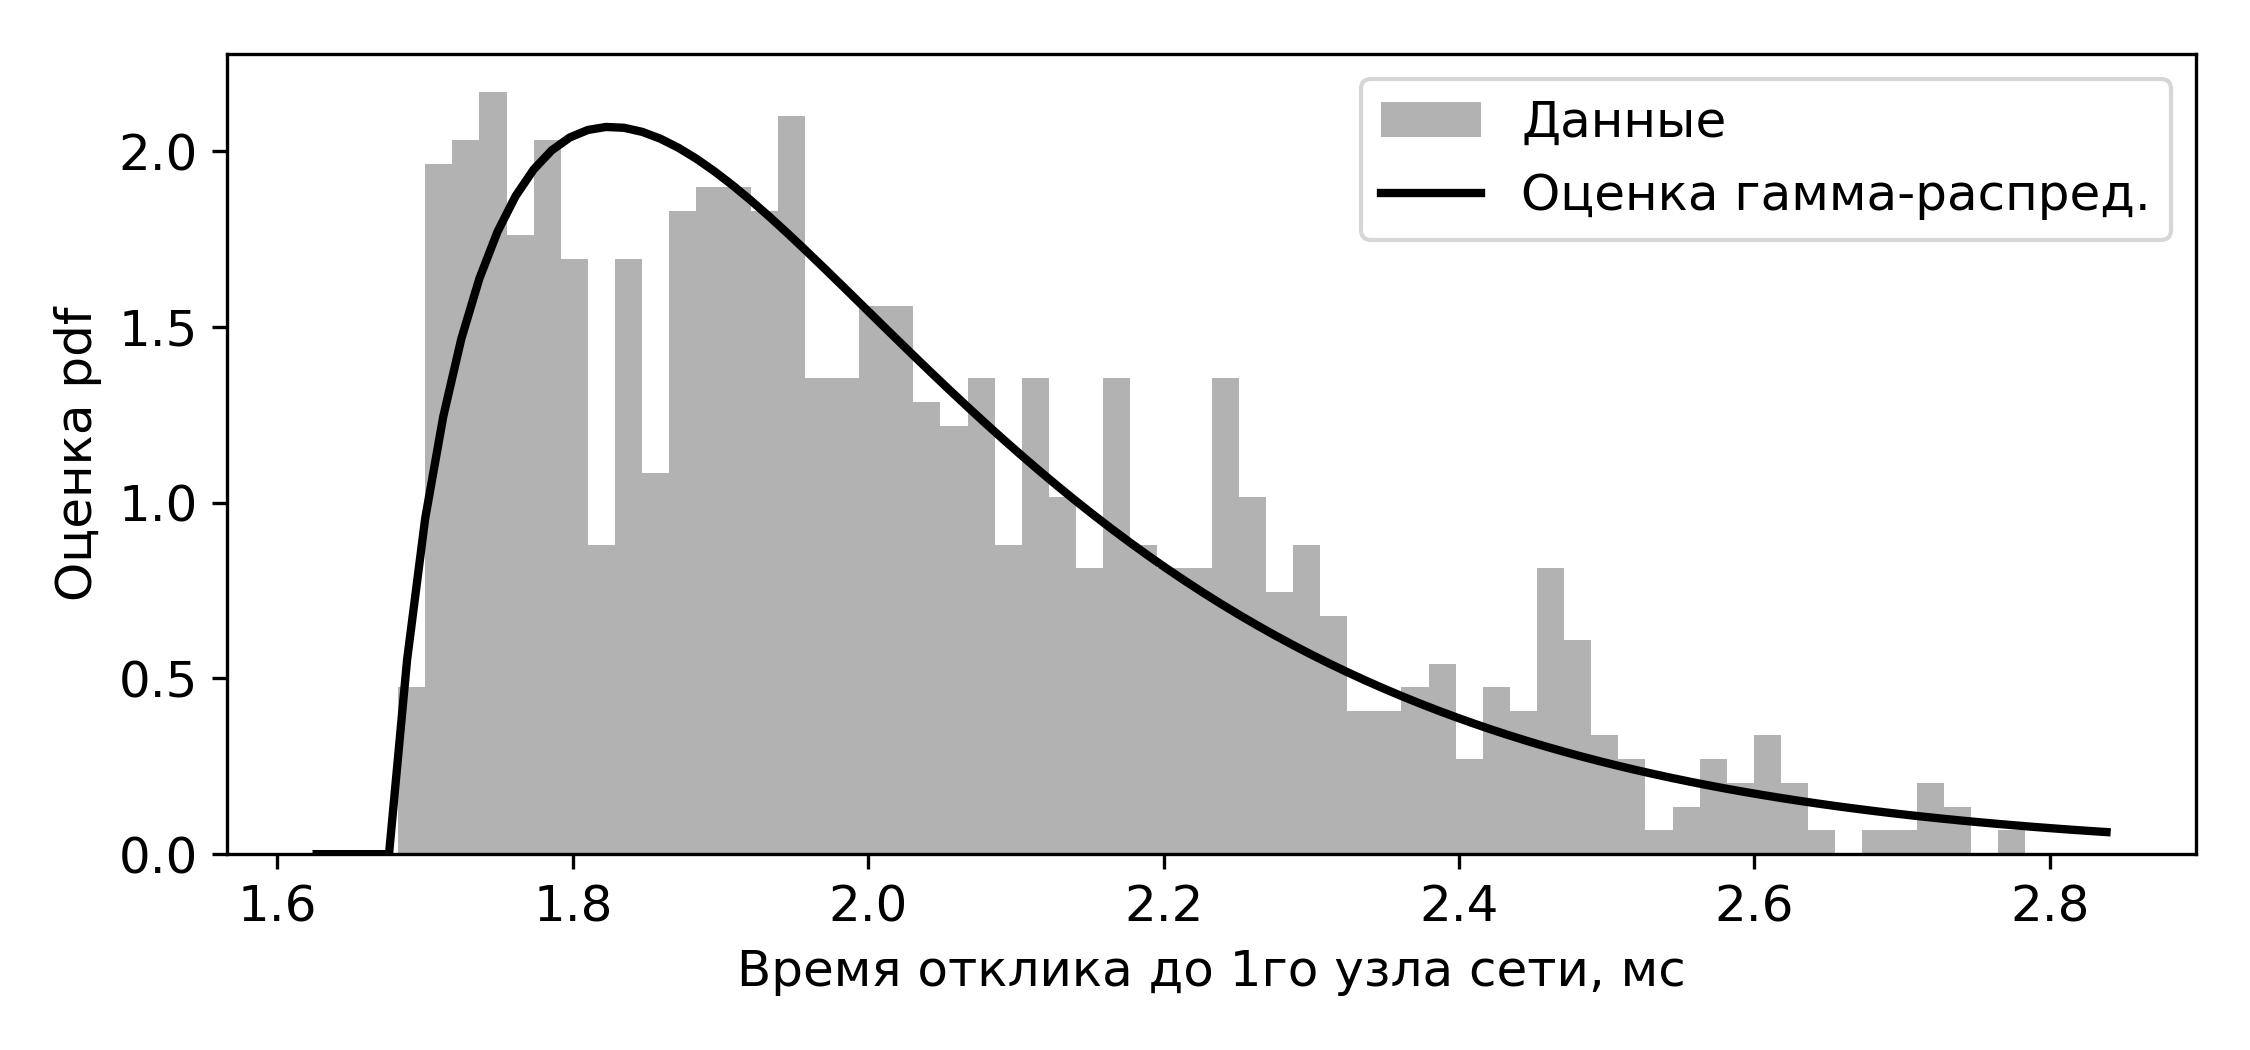
\includegraphics[width=0.7\linewidth]{images/calib/example_kde}
		\caption{Пример получаемого приближения pdf для устройства типа “system: V1” с использованием гамма-распределения}
		\label{fig:examplekde}
	\end{figure}
\end{comment}

После чего для полученных функций распределения проводилась оценка их различий с помощью дивергенции Кульбака-Лейблера, а точнее с помощью ее симметричной версии – дивергенции Джефриса (\ref{jefrice}) \cite{jeffreys}, которая в отличие от KL-дивергенции (\ref{kl_deiv}) является коммутативной операцией.

\begin{equation}
	D_{KL}(P||Q) =  \int_X p \cdot log \frac{p}{q} d\mu
	\label{kl_deiv}
\end{equation}


\begin{equation}
	D_{J}(P||Q) =  \frac{1}{2} D_{KL}(P||Q) + \frac{1}{2} D_{KL}(Q||P) ,
	\label{jefrice}
\end{equation}
где p и q --- функции плотности распределения сравниваемых распределений P и Q.


Согласно Таблице \ref{pdf_compare} наименьшее значение используемых дивергенций у наблюдаемых данных наблюдает при сравнении с логнормальным и гамма распределениями (Рисунок \ref{fig:kderesults}). Полученные наборы расстояний между распределениями для этих двух распределений статистически не отличаются (тест Манна Уитни p-value << 0.05). В связи с этим оба распределения были использованы в дальнейшей работе по проведению калибровки данных.


\begin{table*}[!ht]
	\centering
	\caption{Результаты сравнения наблюдаемых данных и рассматриваемых параметрических распределений, выраженные в
		расстоянии (дивергенции) Джефриса от табличного распределения до оценки по KDE. Обозначения распределений: normal - нормальное, lognormal - логнормальное, skewnorm - смещенное нормальное, gennorm - обощенное нормальное}
	\begin{tabular}{|c|c|c|c|c|>{\centering\arraybackslash}p{2.8cm}|c|}
		\hline
		normal & lognormal & skewnorm & gamma & gennorm & Тип устройства & Лучшее \\ \hline
		1,173 & 0,101 & 0,271 & 0,153 & 0,823 & system: V4 & lognormal \\ \hline
		0,928 & 0,050 & 0,411 & 0,081 & 0,458 & system: V3 & lognormal \\ \hline
		0,161 & 0,026 & 0,531 & 0,018 & 0,064 & Software   & gamma \\ \hline
		0,134 & 0,056 & 0,402 & 0,032 & 0,091 & system: V1 & gamma \\ \hline
		0,340 & 0,066 & 0,167 & 0,022 & 0,603 & system: V2 & gamma \\ \hline
		0,121 & 0,125 & 0,461 & 0,049 & 0,109 & Anchor     & gamma \\ \hline
	\end{tabular}
	\label{pdf_compare}
\end{table*}



\begin{figure}
	\centering
	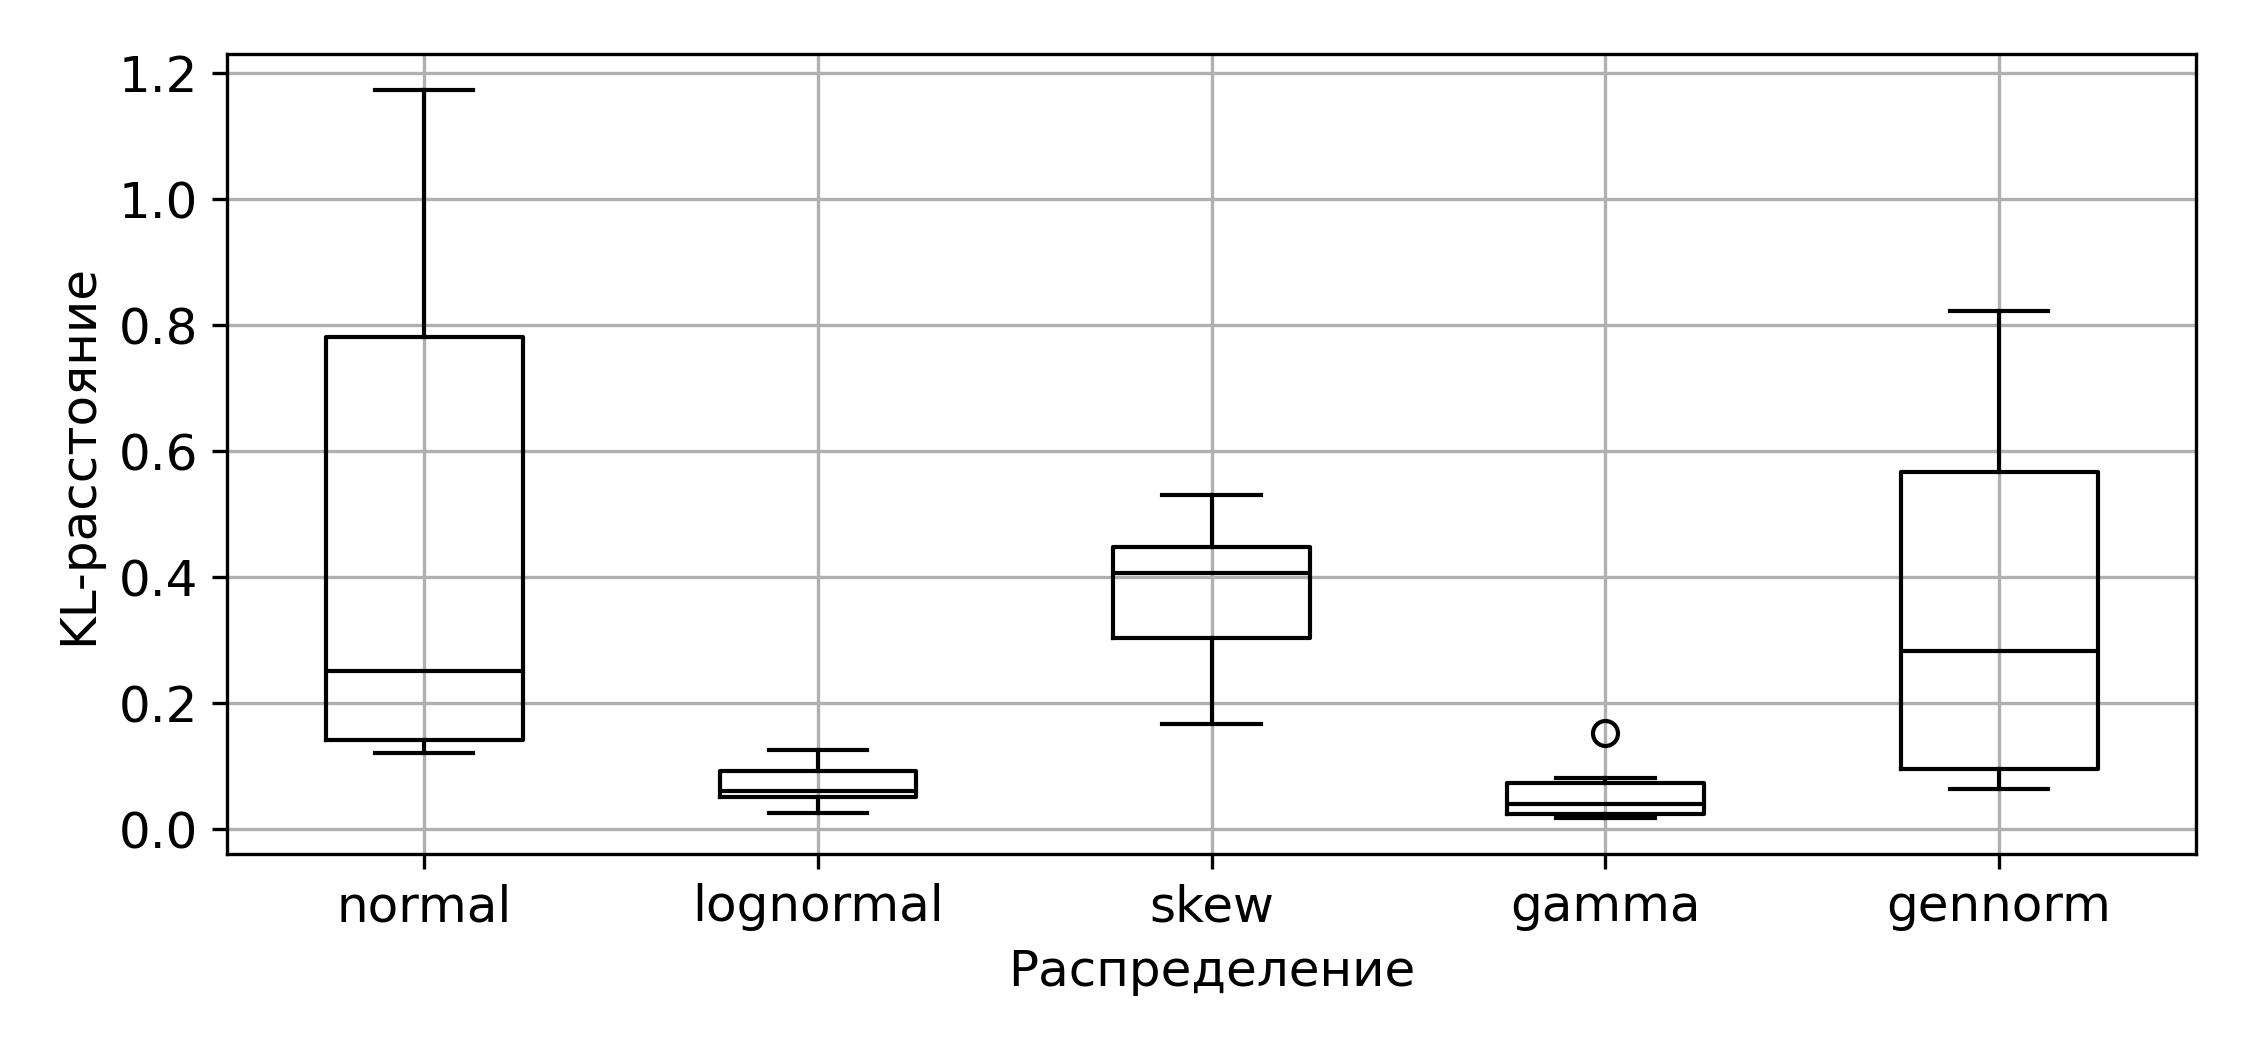
\includegraphics[width=0.7\linewidth]{images/calib/kde_results}
	\caption{Результаты сравнения KDE наблюдаемых данных и рассматриваемых параметрических распределений}
	\label{fig:kderesults}
\end{figure}


\subsection{Применения калибровки с использованием полученной оценки функции распределения}\label{subsec:ch3/sect5/sub2}

Для проведения калибровки была исследована возможность применения подхода с использованием преобразования распределений, то есть переноса данных из одного вероятностного пространства в другое. Для этого полученные ранее измерения преобразовывались по следующей формуле:

\begin{equation}
	x_{calib} = F_{ref}^{-1}(F_{obs}(x)) , 
	\label{сalib_table}
\end{equation}
где $F_{ref}^{-1}$ - это обратная функция распределения для времени отклика эталонного устройства, а $F_{obs}$ - функция распределения для времени отклика калибруемого зонда. Обе функции получаются путем использования параметрического распределения. Выбор используемого семейства распределений
обосновывается результатами предыдущего раздела. 

Как уже было обосновано в разделе \ref{sec:ch3/sect2}, версия устройств <<system: V3>> рассматривалось как эталонное. Также стоит подчеркнуть, что ряд работ подчеркивает более высокую аппаратную мощность данного поколения устройств \cite{Bajpai2015}. Пример подобной калибровки приведен на Рисунках \ref{fig:before_gamma} и \ref{fig:after_gamma}.

\begin{figure}[ht]
	\centerfloat{
		\hfill
		\subcaptionbox[List-of-Figures entry]{До проведения калибровки\label{fig:before_gamma}}{%
			
\includegraphics[width=0.49\linewidth]{calib/before_gamma}}
		\hfill
		\subcaptionbox{После калибровки с использованием гамма-распределения \label{fig:after_gamma}}{%
			
\includegraphics[width=0.49\linewidth]{calib/after_gamma}}
		\hfill
	}
	\caption{Данные с устройств <<system:V4>> и <<system:V3>>}\label{fig:before_after_gamma}
\end{figure}



Описанный метод использовался как с применением логнормального и гамма распределений, после чего сравнивался с методом, описанным в разделе \ref{sec:ch3/sect2}.
Анализ результатов калибровки был проведен с помощью двух метрик: расстояния Джефриса и 1-е Вассерштейна (\ref{eq:wass}) \cite{wass_1}, \cite{Ramdas2017} до выбранного эталонного устройства. Метрика Вассерштейна была добавлена в анализ, так как она учитывает геометрическое расстояние между распределениями и чувствителен к сдвигам, растяжениям и другим пространственным изменениям \cite{wass_1}. Также в рассмотрение был добавлен метод, базирующийся
на предположении, что дополнительная задержка постоянна, и может быть вычислена исходя из разницы медиан описанный в разделе \ref{sec:ch3/sect2}.


\begin{equation}
	W_1(P,Q) = \int_{-oo}^{+oo} |P(x)-Q(x)|dx ,
	\label{eq:wass}
\end{equation}
где $P(x)$ и $Q(x)$ – это функции распределения, вместо которых в библиотеке scipy используются эмпирические функции распределения (Empirical Cumulative Distribution Function — ECDF) \cite{wass_2}.

Для устройств версии V1, V2 и V4 обе метрики показывают значимое снижение расстояния для всех трех рассматриваемых методов калибровки (Рисунки \ref{fig:kl1}- \ref{fig:was1}).


\begin{figure}
	\centering
	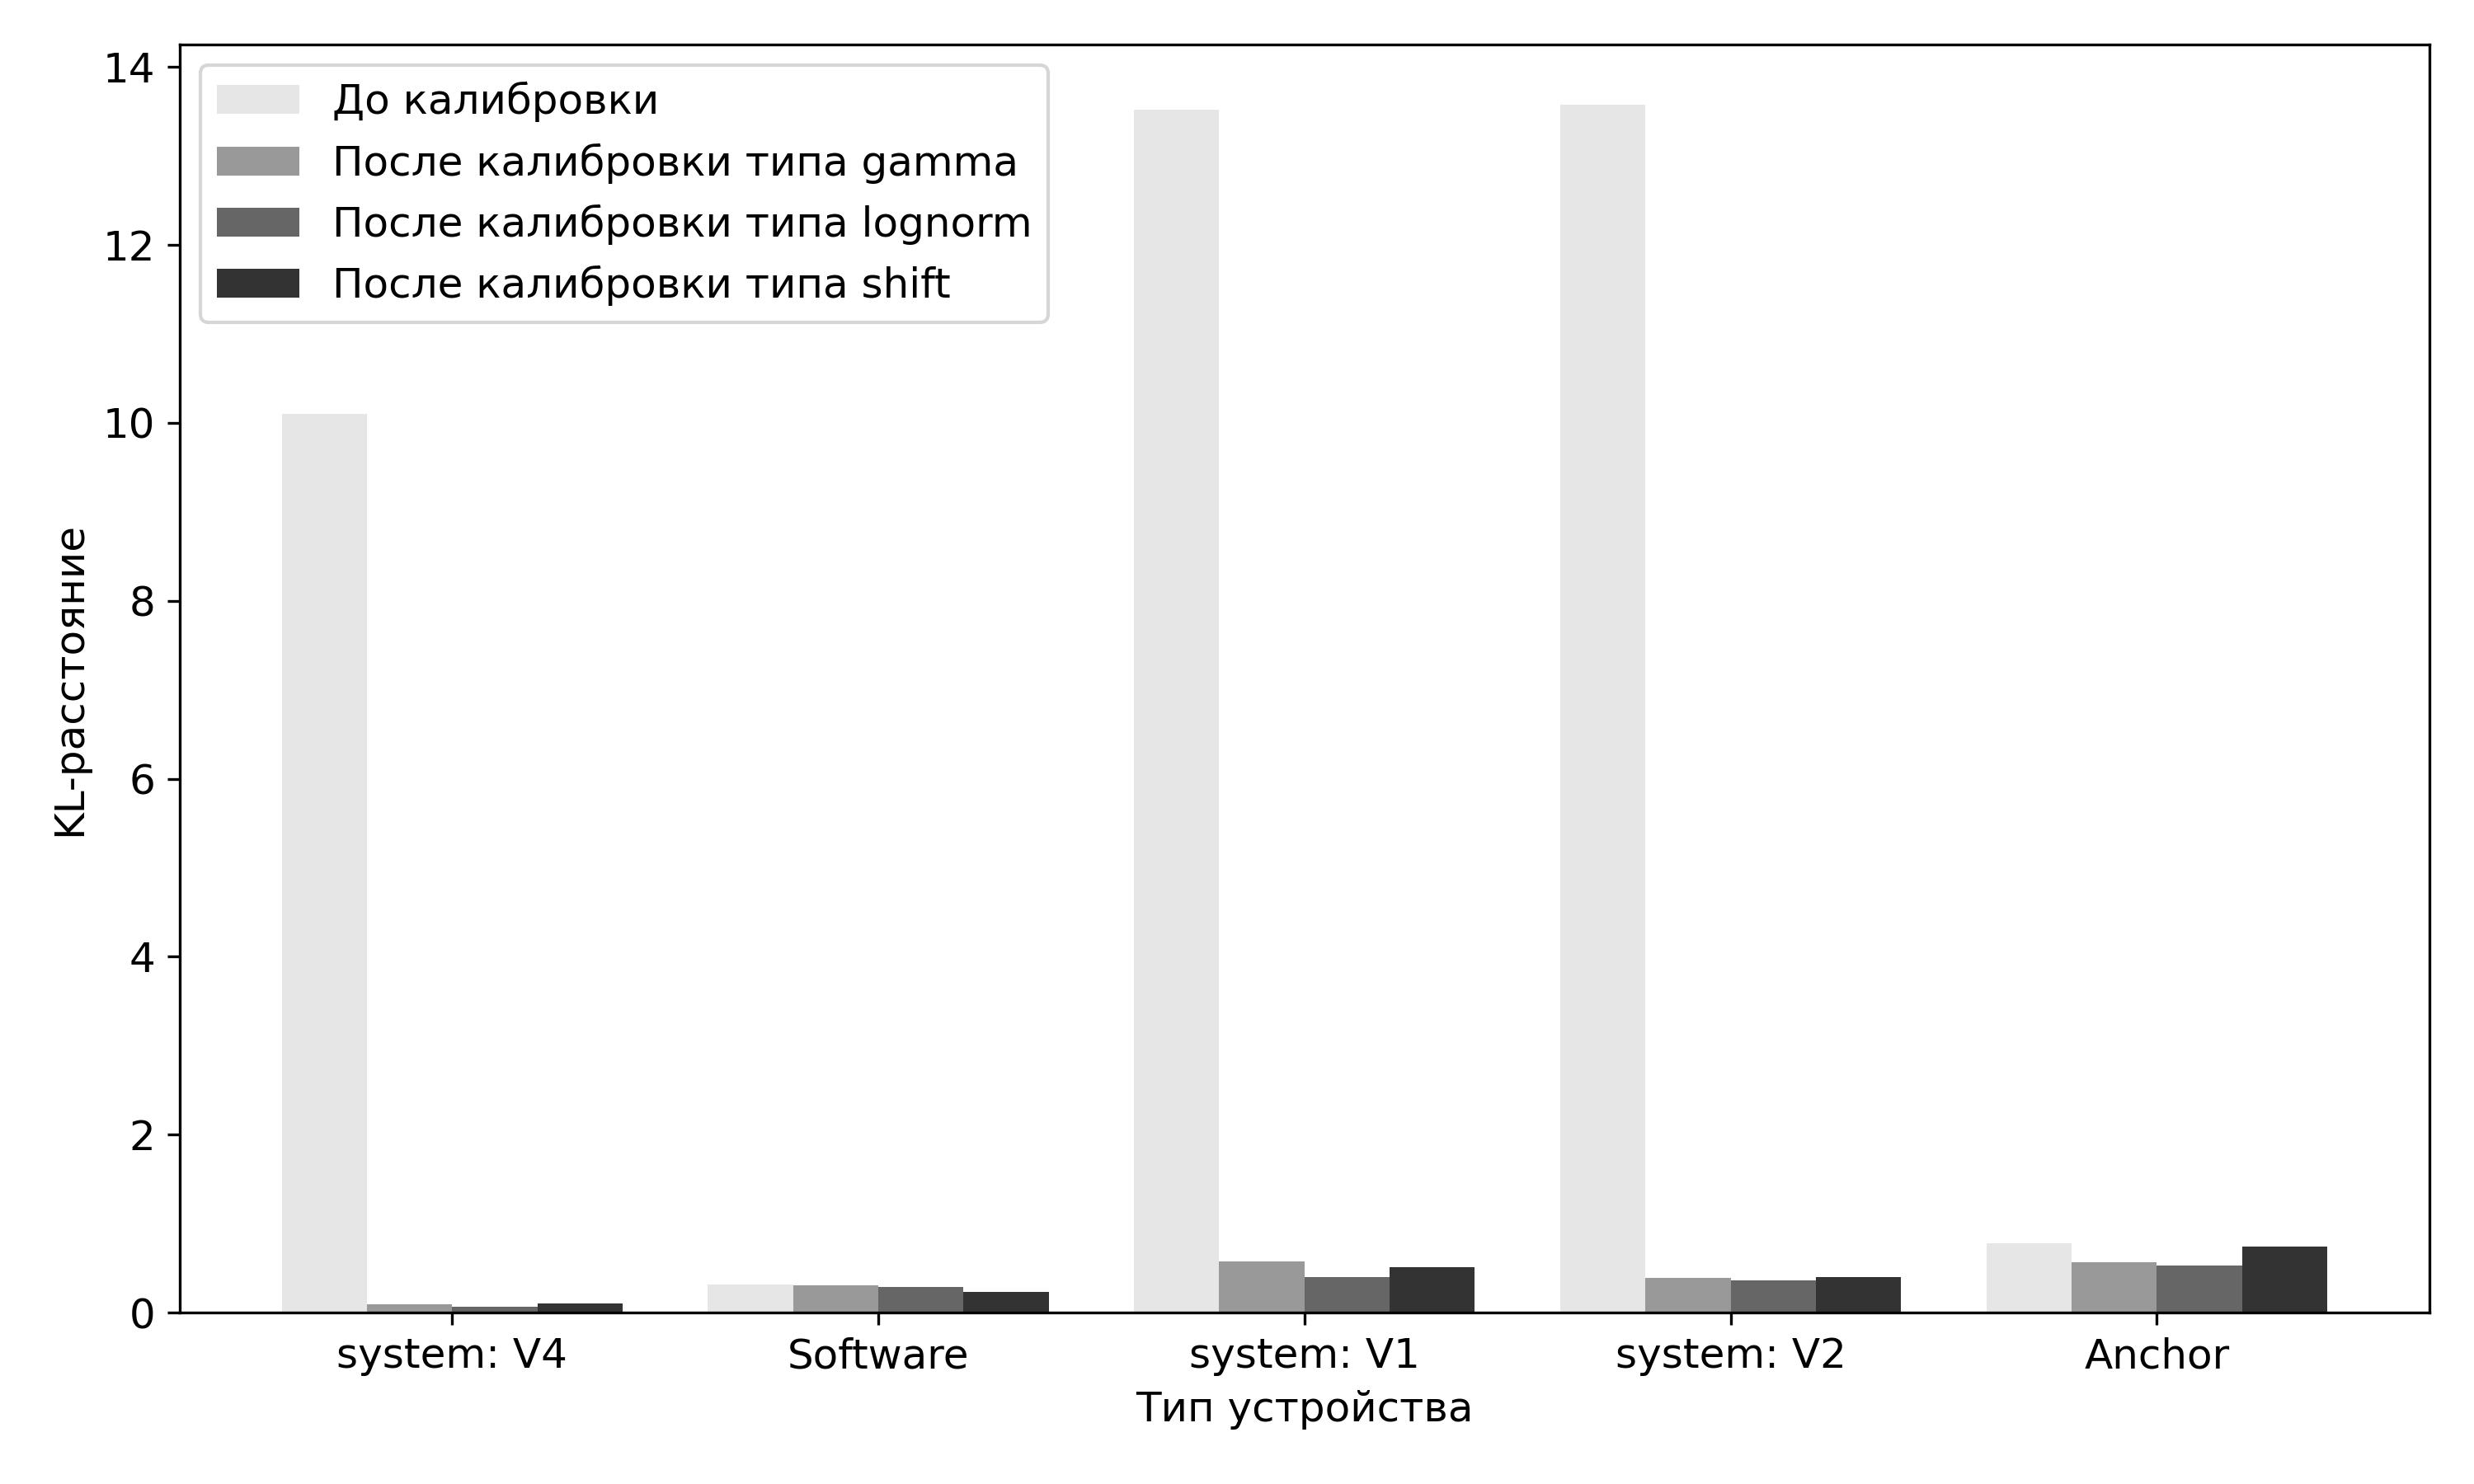
\includegraphics[width=1.0\linewidth]{../images/calib/KL_1}
	\caption{Сравнение дивергенции Джефриса до и после применения калибровки}
	\label{fig:kl1}
\end{figure}

\begin{figure}
	\centering
	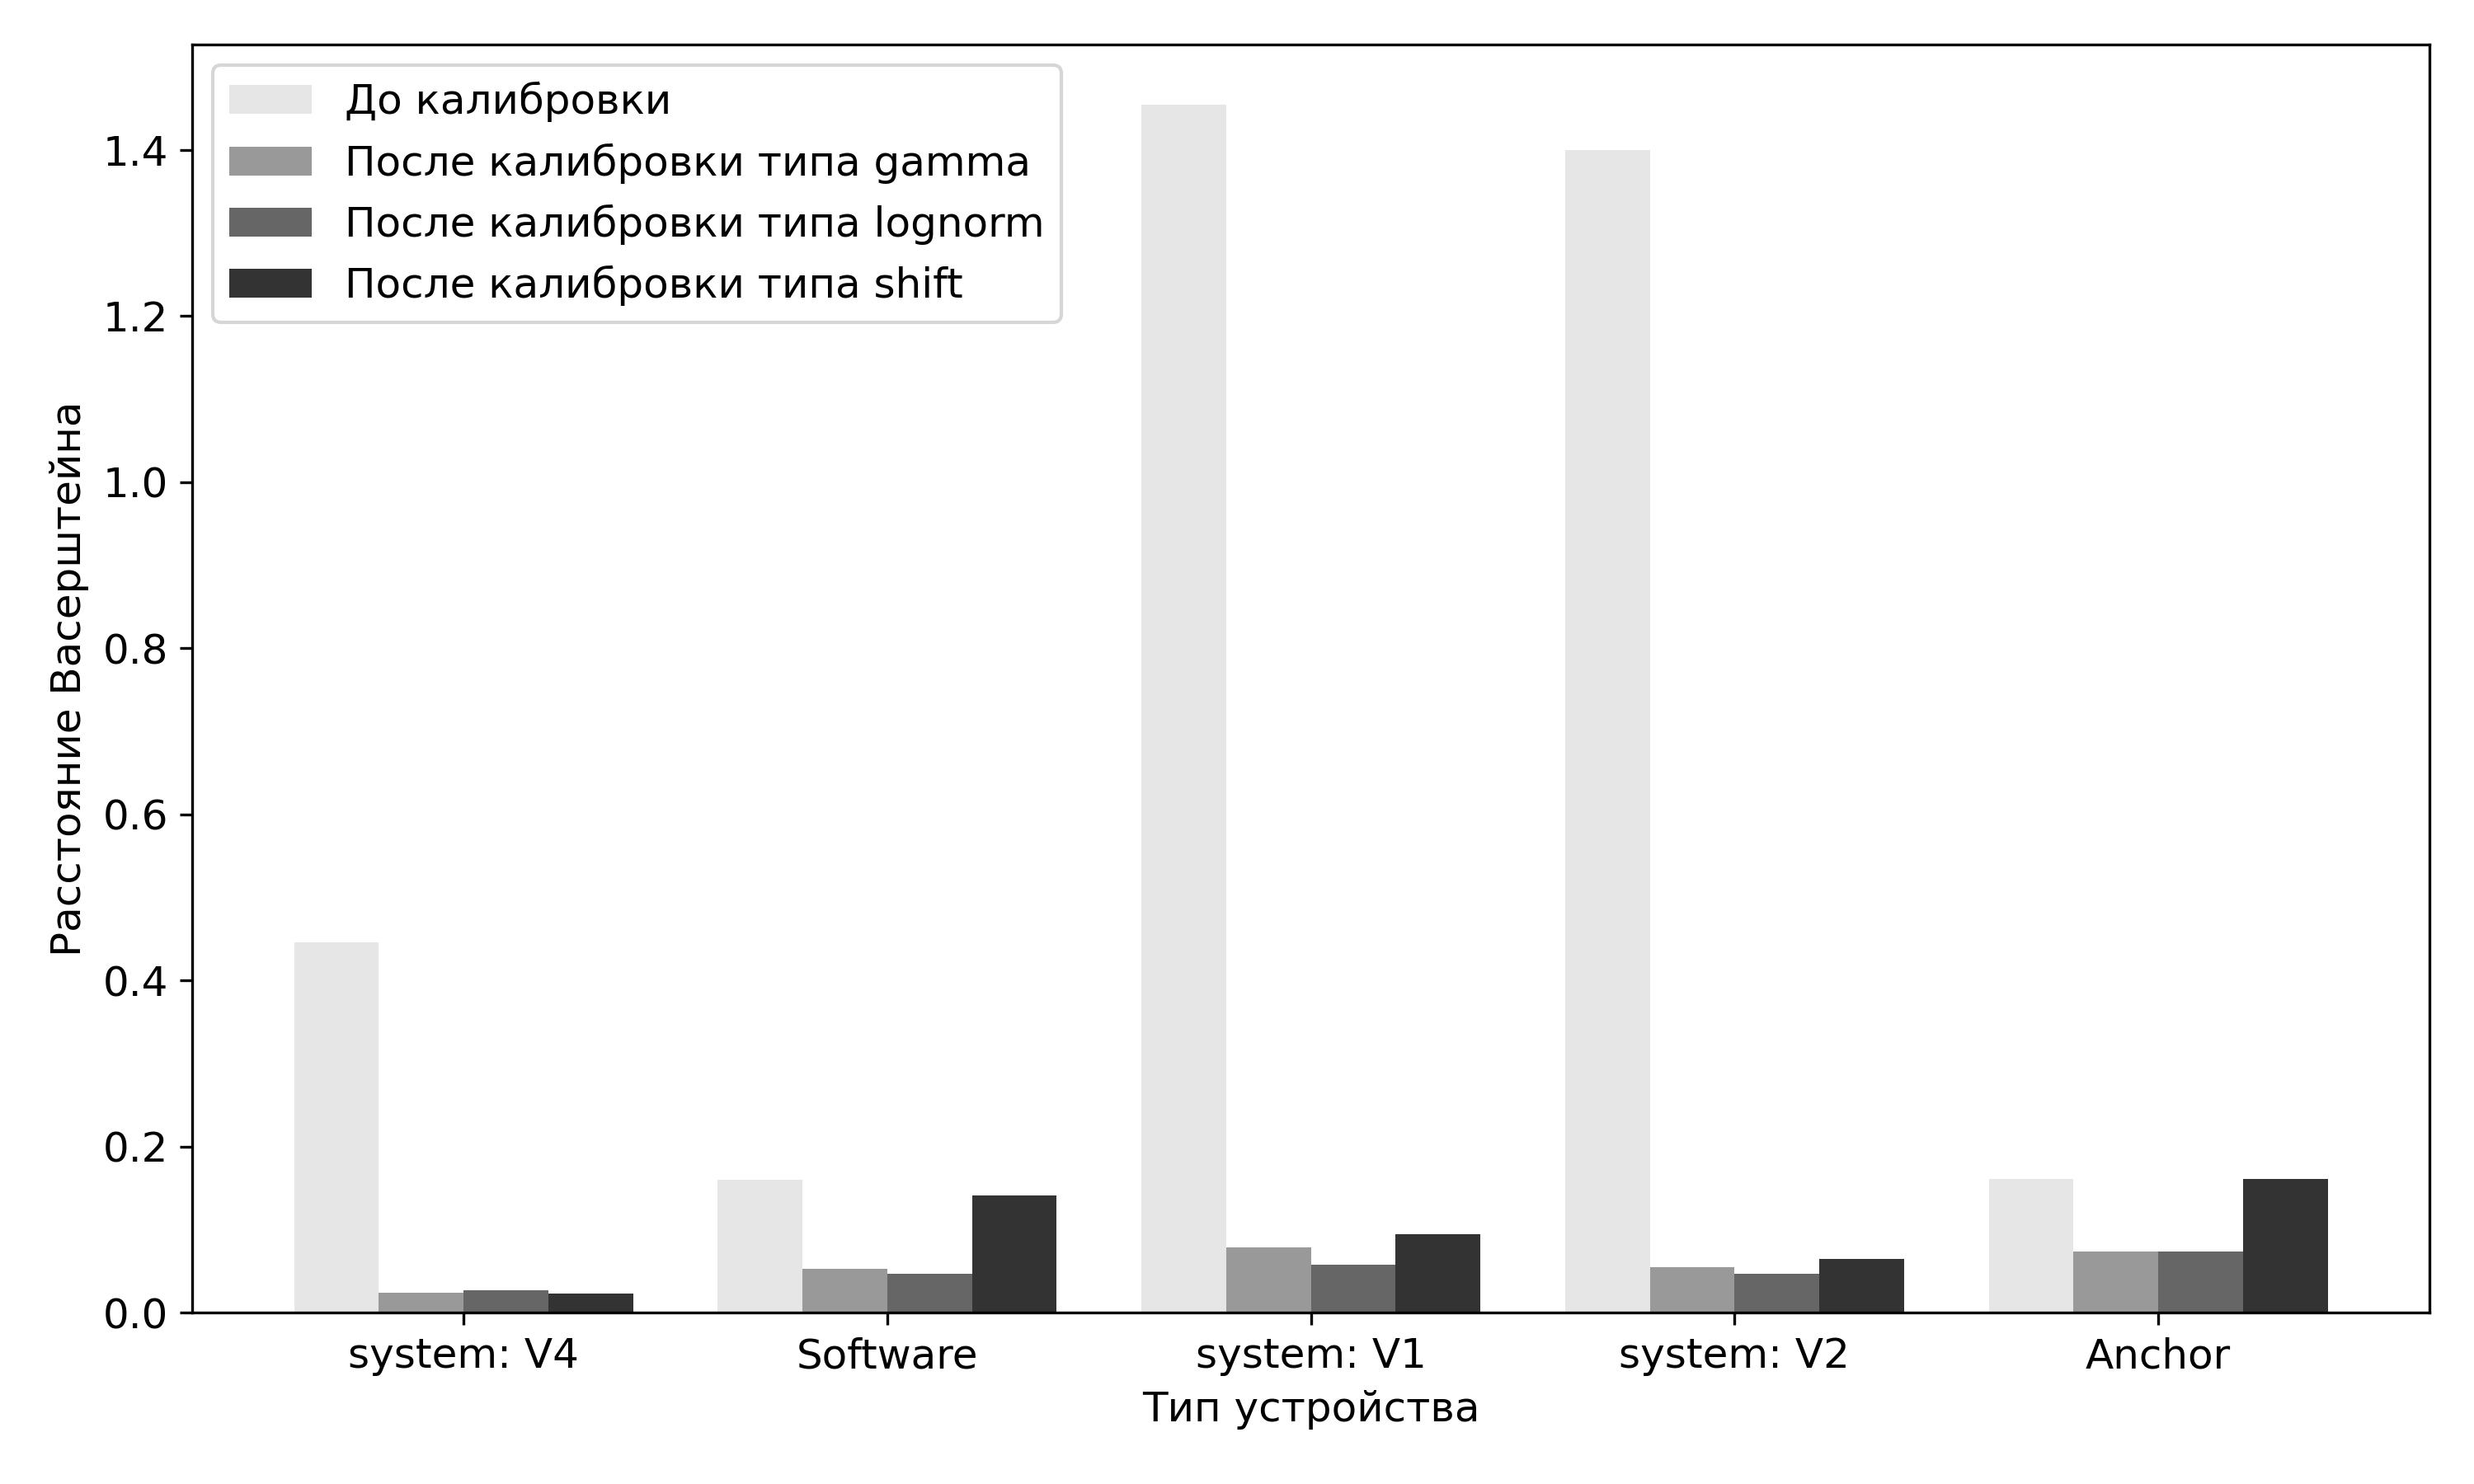
\includegraphics[width=1.0\linewidth]{../images/calib/was_1}
	\caption{Сравнение Расстояния Вассерштейна до и после применения калибровки}
	\label{fig:was1}
\end{figure}


При подробном рассмотрении метрик (Рисунок \ref{fig:kl1}- \ref{fig:was2}) можно отметить, что для устройств типа <<Software>> и <<Anchor>> результаты разнятся в зависимости от применяемой метрики и используемого метода калибровки. Например, можно отметить, что использование подхода преобразования распределений демонстрирует большее снижение расстояния Вассерштейна в сравнении с методом сдвига.
Это можно связать с тем, что распределения этих двух устройств значимо отличаются по форме. В итоге метод сдвига снижает обе рассматриваемые метрики, однако преобразование распределений делает это кратно лучше на устройствах типа <<Software>> и
<<Anchor>> (разница расстояний Вассерштейна до и после калибровки для типа Anchor увеличилась в сотни раз, для Software более чем в 5 раз), что
позволяет сделать вывод о большей точности разработанного метода в рамках расстояния между распределениями.

Метод калибровки был реализован на языке программирования Python. Основной фрагмент представлен в Листинге \ref{lst:calib} в Приложении \ref{app:A}


\begin{figure}
	\centering
	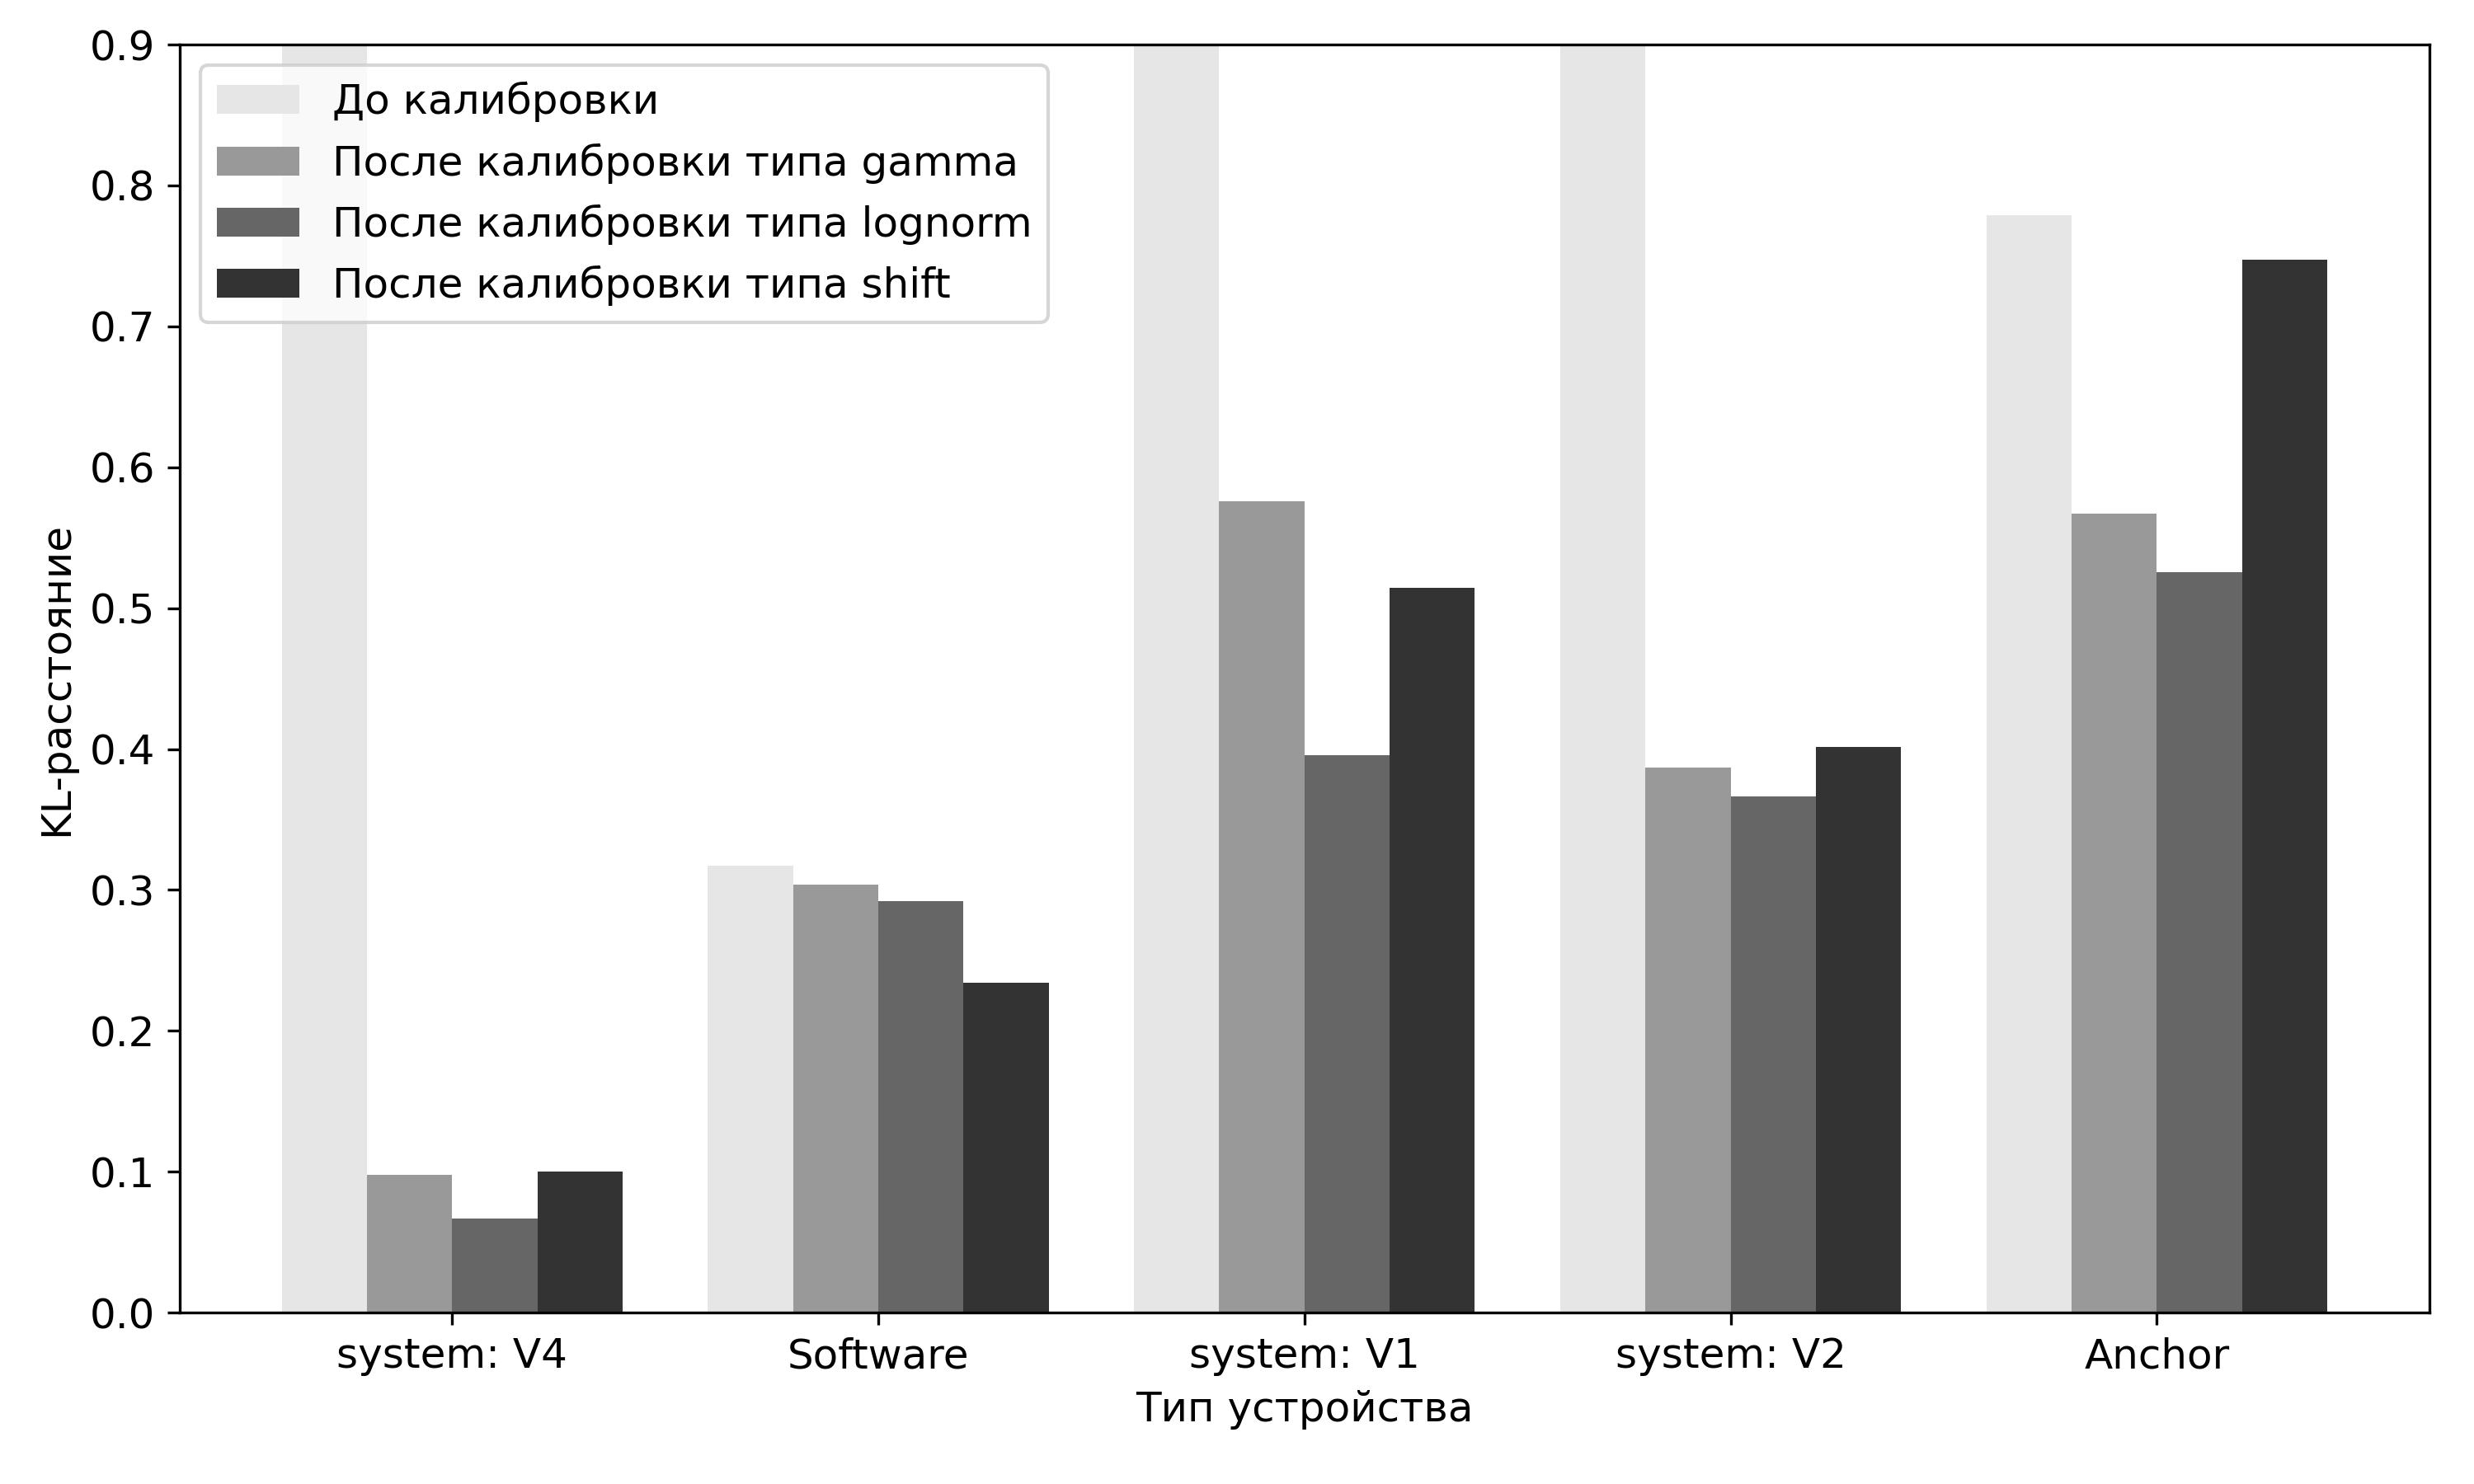
\includegraphics[width=0.7\linewidth]{../images/calib/KL_2}
	\caption{Сравнение дивергенции Джефриса до и после применения калибровки (увеличенный масштаб)}
	\label{fig:kl2}
\end{figure}


\begin{figure}
	\centering
	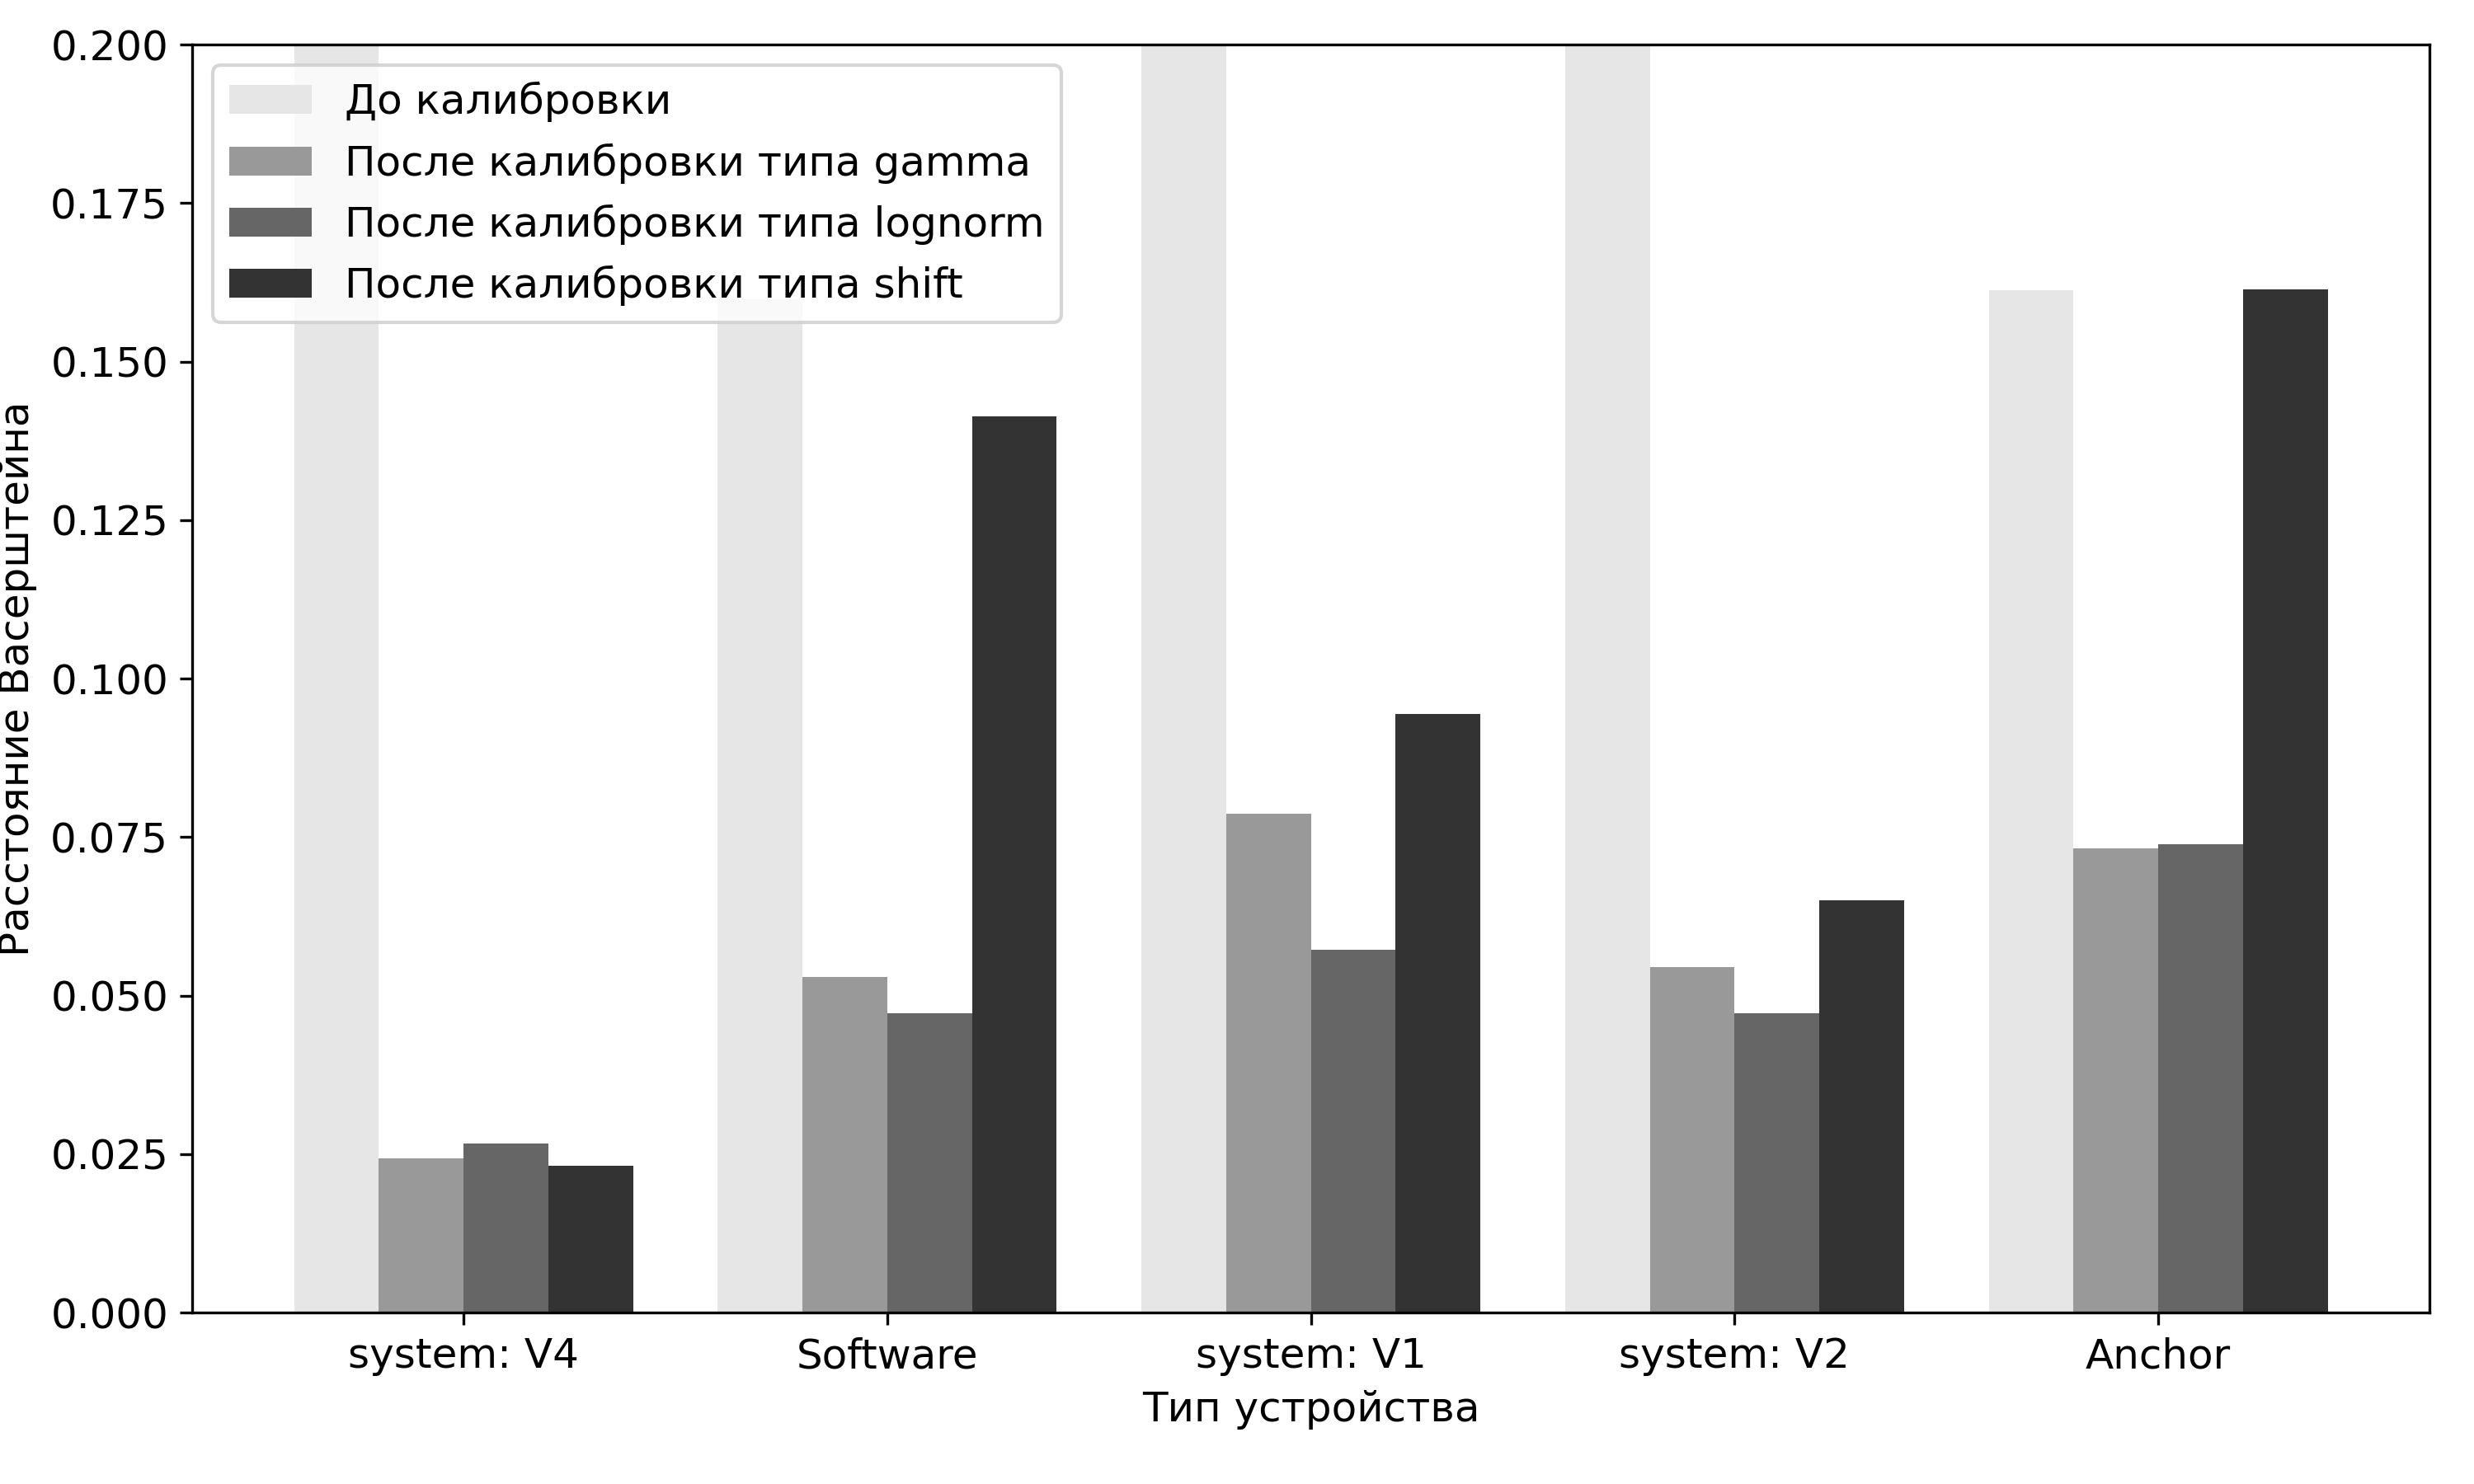
\includegraphics[width=0.7\linewidth]{../images/calib/was_2}
	\caption{Сравнение расстояния Вассерштейна до и после применения калибровки (увеличенный масштаб)}
	\label{fig:was2}
\end{figure}


%\section{Преобразование распределений с использованием современных архитектур нейронных сетей }\label{subsec:ch3/sect6}


%Normalizing Flows — это класс моделей, которые позволяют эффективно моделировать сложные распределения вероятностей путем применения последовательности обратимых трансформаций к простому распределению, например, нормальному. Эти модели обеспечивают гибкость в представлении данных и могут быть использованы для генерации новых образцов из обученного распределения.


%Использование моделей нормализующих потоков (Normalizing Flows) для калибровки показателей представляет собой перспективный подход в области машинного обучения и статистики. Ниже приведено объяснение основных идей и методов, которые могут быть использованы для этой цели....

\section{Выводы по 3 главе}\label{subsec:ch3/sect7}


В главе \ref{ch:ch3} был предложен новый метод калибровки данных о производительности сети, полученных из системы RIPE Atlas. Метод основан на оценке наблюдаемых картин распределений и их последующем преобразовании. 
Проведенные исследования показали, что лучше всего полученные данные времени отклика до 1го узла сети описываются гамма и логнормальным распределениями. Результаты также показали, что разработанный подход калибровки в ряде случаев превосходит метод оценки систематической ошибки, а в остальных демонстрирует сопоставимую эффективность. Наибольшие изменения метод показал в метрике расстояния Вассерштейна, что подтверждает его перспективность для задач, связанных со значимым различием форм распределений.

Однако стоит подчеркнуть, что для разработанного метода есть пространство для улучшений и оптимизации. Так, в дальнейшие планы исследований входят:

\begin{itemize}
	\item Проведение более масштабные экспериментальных исследования на более разнородных данных для оценки устойчивости метода при росте географических масштабов и появлении новых поколений устройств.
	\item Исследование условий сходимости и оптимальности метода.
	\item Адаптация метод для работы с многомерными распределениями и
	потоковыми данными.
	\item Исследование возможность комбинирования нового метода с другими
	подходами к калибровке для повышения точности.
\end{itemize}

Выполнение данных аспектов в дальнейшем исследовании позволит углубить понимание предложенного метода и расширить область
его практического применения на различные потенциальные сценарии, связанные с измерениями времени отклика в распределенных системах измерений.


\FloatBarrier
%\clearpage
